\documentclass{IEEEtran}
\usepackage{graphicx}
\usepackage{hyperref}

\graphicspath{ {./images/} }

\title{Food/Non-Food Classification}
\author{Jaime Garcia Diaz (jaimeg4@illinois.edu), Faizan Khan (fkhan71@illinois.edu)}
\date{2021}


\begin{document}

\begin{titlepage}
\maketitle
\end{titlepage}


\begin{abstract}
There's a continuous growing interest in eating healthier that has made available a lot of digital content that provides nutrition facts about the food we eat. At the same time the field of image recognition and data classification has caught the attention of a great number of data scientist enthusiasts and there are multiple papers and projects that have done work on the subject.\\\\

We report the experiment of food / non-food classification using cloud technologies. The experiment will perform on dataset Food- 101.\\
\end{abstract}

\textbf{Keywords}\\
Classification; food/non-food; CNN\\

I. INTRODUCTION\\

In this technology time, the dietary assessment has been seen a lot of development. One of the major components of dietary assessment is food classification. There has been lot of development in image processing and recognition task.\\

There are some problems which are still difficult to resolve like highly mixed food items in a plate, so we decided to solve general type of certain food in this paper.\\

This paper drive two types of experiments.\\
\begin{itemize}
\item Food vs non-food classification (binary)

\item Food category recognition\\

\end{itemize}


II. DATASET\\


The \href{https://registry.opendata.aws/fast-ai-imageclas/}{Food-101} will be used for this experiment. The Food-101 dataset is having 101 food categories. Per category it is having 750 training and 250 test images.\\

III.APPROCAH \\

After going through the open data on AWS we have chosen to work with the Food-101 dataset, which has been cited a couple of times in multiple interesting papers that will help to get pieces of the project. However, the part that the papers don’t cover as much, is about making the Food/Non-Food classification in real time.\\

The intention of the project is to implement the following module:\\

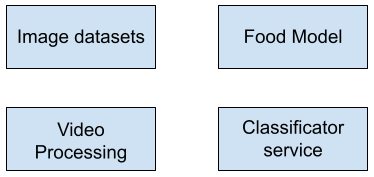
\includegraphics[scale=0.5]{modules}\\

\begin{itemize}
\item \textbf{Image dataset}.
Use a couple of the public datasets and complement them with images from Instagram. 

\item \textbf{Food Model}.
Train a model and so that it could classify images.

\item \textbf{Video Processing}.
Process a video stream into frames, such that the frames could be classified.

\item \textbf{Classification service}.
Setup a service that uses the previous modules and classifies a video feed in real time.\\
\end{itemize}


As potential future work, the real time classification could be enhanced by detecting the type of food (ie. pizza or salad, etc.) and while it might be hard to show the actual nutrition facts, at least it should be feasible to display a generic reference for the type of food in the feed.\\


IV. LITERATURESURVEY\\

Food image classification and recognition are very popular topic in image processing. Lot of research papers are published for this problem.\\

The first problem is to detect image that contains the food item so, task of food/non-food is binary classification problem. When we feed an image to system then it identifies whether image is food or non-food.\\

The Convolutional Neural network provides an approach for an image classification and recognition problem.\\
Kagaya [1] used CNN in food vs non-food classification.
It achieved 93.8% accuracy.\\

Another work [2] where the accuracy of food vs non-food improved to 99.1%. If we compare with other works, the CNN provide superior performance.\\

CNN is most popular network used in food recognition and provide better result compare to conventional methods. Bossard [3] trained a CNN on food-101 dataset and achieved 56.4 top-1 accuracy.\\

In [1] paper, also trained CNN for food recognition and achieved Better result than the other classical approach by achieving 73.7 accuracy.\\

In papar[4], GoogLeNet model was used to classify food/non- food images.\\

It also categorizes food into 11 below categories\\

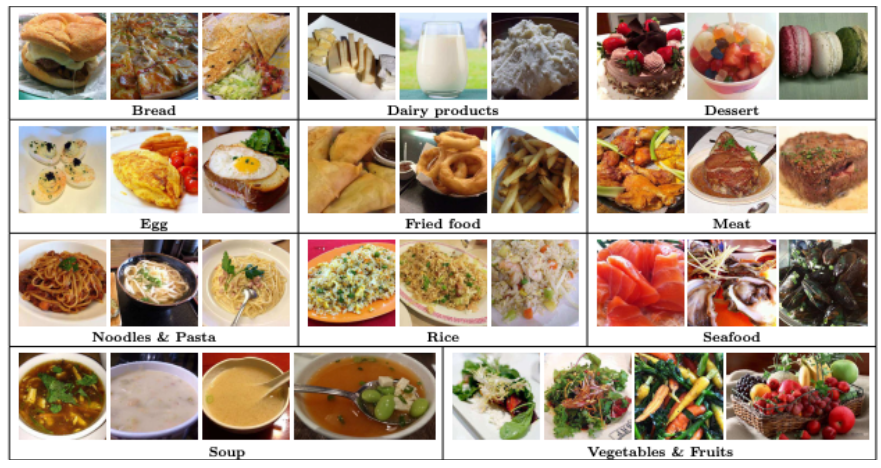
\includegraphics[scale=0.2]{food}\\

GoogLeNet is efficient deep learning model architecture.\\

The Food-5k dataset used for this study and which contains around 2500 food images and 2500 nonfood images. Below is experiment result of paper.\\

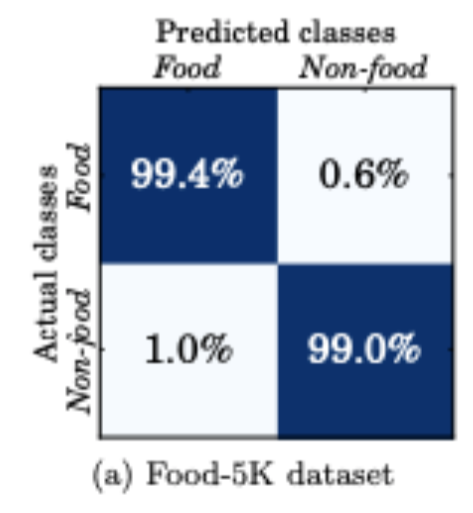
\includegraphics[scale=0.5]{classes}\\

There is lot of work in image classification and recognition. In this paper we will use cloud technology to achieve food classification.\\


V. REFERENCES\\

[1] https://dl.acm.org/doi/10.1145/2647868.2654970\\

[2] https://link.springer.com/chapter/10.1007/978-3-319\\

[3] Lukas Bossard, Matthieu Guillaumin, and Luc Van Gool. Food-101 – mining discriminative components with random forests. In European Conference on Computer Vision, 2014.\\

[4] \href{https://www.researchgate.net/publication/310823982_FoodN on-
food_Image_Classification_and_Food_Categorization_using _Pre-Trained_GoogLeNet_Model}{Food/Non-food Image Classification and Food Categorization using Pre-Trained GoogLeNet Model
}\\

[5] \href{https://www.ijstr.org/final-print/mar2020/An-Efficient-Food-Image-Classification-By-Inception-v3-Based-Cnns.pdf}{An Efficient Food Image Classification By Inception- V3 Based Cnns}\\


[6] \href{https://link.springer.com/content/pdf/10.1007/978-3-319-23222-5_43.pdf}{Highly Accurate Food/Non-Food Image Classification Based on a Deep Convolutional Neural Network}\\

[7] \href{https://www.researchgate.net/publication/309128470_Food_Image_Recognition_Using_Very_Deep_Convolutional_Networks}{Food Image Recognition Using Very Deep Convolutional Networks}\\

[8] \href{https://www.ijert.org/research/human-face-recognition-using-image-processing-IJERTCONV2IS04051.pdf}{Facial Recognition System Using Image Processing}\\\\

\textbf{About the authors:}\\




\begin{itemize}
\item Faizan Ali Danish Khan is student in UIUC and currently pursuing master’s in computer science.\\

\item Jaime Garcia Diaz is student in UIUC and currently pursuing master’s in computer science.\\
\end{itemize}







\end{document}